% esm4124_f04_forestwalker.tex
% group report for an ESM 4124 group project
% 2004.12.11

\documentclass{article}
%\usepackage[pdftex]{graphics}
\usepackage{graphicx}
%\usepackage{fancyhdr}
\usepackage{amssymb,amsmath}
\begin{document}

\title{ESM 4124 Group Project \\ Forest Walker}
\author{Alpha Chen, Ricky Franklin, Khang Le}
\maketitle

\begin{abstract} %{{{
U.S. Patent 6,109,378 describes a leg mechanism used in a walking forest machine. Technical difficulties in creating an animation of the forest walker include creating the walker model and then expressing the animation through state variables which change with time. These problems were overcome by applying the knowledge gained in the course to each problem. A model was created, animated through kinematics, and the animation finished with our knowledge of dynamics.

The animation must show the forest walker walking on a slope, collecting trees for harvest. The walker must then drop a harvested tree down a slope, demonstrating dynamic motion of an isolated rigid body with forces describing its position and orientation.
\end{abstract}%}}}

\section{Constituent Rigid Bodies} %{{{

The forest walker consists of its body, six legs, and the grabber mechanism. To ease the process of developing a model, these parts were created and modeled independently before creating the final model.

\subsection{Main Body}%{{{
As the body of the forest walker cannot change shape, it can be considered a single rigid object. Because the body is unconstrained, it has six configuration coordinates.%}}}

\subsection{Leg Mechanisms}%{{{
The forest walker has a total of six legs. For simplicity, all the legs are considered to be exact copies of each other. This allows us to model one leg and apply that model to create the other legs. Although the leg mechanism described in the patent is complex, it can be reduced to three main sections for ease in modeling. The upper arm of the leg connects the leg to the body of the walker, and is thus translationally constrained. The lower arm connects the upper arm to the foot of the leg. With three degrees of freedom for translating the upper arm to the correct location relative to the body of the walker, two degrees of rotational freedom for the upper arm, one for the lower arm, and two for the foot, each leg uses eight configuration coordinates. Therefore, all six legs will require forty-eight configuration coordinates.%}}}

\subsection{Grabber Mechanism}%{{{
The forest walker must be able to cut down trees for logging. This is where the grabber mechanism comes into play; it is attached to an arm which extends from the top of the body. The arm consists of three segments; the base segment has two degrees of rotational freedom, and the other two have a single degree of rotational freedom each. Attached to the end of the last segment is the actual tree grabber, with one degree of rotational freedom. Thus, the entire mechanism has five degrees of freedom.%}}}

\subsection{Tree}%{{{
Although not a part of the forest walker, the dropped log at the end of the animation is represented as a cylinder with a full six degrees of freedom.%}}}
%}}}

\section{Reference Points and Reference Triads} %{{{

\subsection{Main Body } %{{{
Let the reference point $A_{Body}$ be located in the center of the walker body, with the reference triad $a^{(body)}$ be oriented such that $a_2^{(body)}$ runs from the bottom through the top of the main body and $a_3^{(body)}$ from the back to the front of the body.%}}}

\subsection{Leg Mechanism} %{{{
Each leg mechanism consists of three parts, each of which with its own reference point and triad. As there are six legs in total, these reference points and triads will be duplicated for each of the legs.

\subsubsection{Upper Arm}%{{{
The upper arm has a reference point $A_{UpperArm}$ located at the point of contact with the body. The reference triad $a^{(upperarm)}$ is oriented such that $a_3^{(upperarm)}$ runs through the upper arm from the body to the lower arm and $a_2^{(upperarm)}$ is perpendicular to the plane of the entire leg.%}}}

\subsubsection{Lower Arm}%{{{
The reference point $A_{LowerArm}$ is positioned at the point of contact between the lower arm and the upper arm with the reference triad $a^{(lowerarm)}$ oriented such that $a_3^{(lowerarm)}$ runs through the lowr arm from the upper arm to the foot and $a_2^{(lowerarm)}$ is the same as $a_2^{(upperarm)}$.%}}}

\subsubsection{Foot}%{{{
Let $A_{Foot}$ be located at the end of the lower arm, where the foot is connected. $a^{(foot)}$ is chosen such that $a_3^{(foot)}$ is perpendicular to the ground.%}}}
%}}}

\subsection{Grabber Mechanism} %{{{
The grabber arm consists of three parts. Each of these parts move, and therefore require reference points and reference triads.

\subsubsection{Grabber Segment 1}%{{{
The reference point $A_{Arm1}$ is located at the base of the arm, where it connects to the body of the walker. The reference triad $a^{(arm1)}$ is chosen such that $a_3^{(arm1)}$ is parallel to this segment of the arm.%}}}

\subsubsection{Grabber Segment 2}%{{{
Let the reference point $A_{Arm2}$ be located at the base of the segment, where it joins with Segment 1. The reference triad $a^{(arm2)}$ is chosen such that $a_3^{(arm2)}$ runs parallel to the segment and $a_1^{(arm2)}$ is the axis of rotation between Segments 1 and 2.%}}}

\subsubsection{Grabber Segment 3}%{{{
This segment has its reference point $A_{Arm3}$ located at the base, where it connects to Segment 2. Like Segment 2, $a^{(arm3)}$ is chosen such that $a_3^{(arm3)}$ runs parallel to the segment and $a_1^{(arm3)}$ is the axis of rotation between Segments 2 and 3.%}}}

\subsubsection{Tree Grabber}%{{{
Let the reference point $A_{Grabber}$ be located in the center of the actual mechanism that grabs and cuts trees. The reference triad $a^{(grabber)}$ is chosen such that $a_3^{(grabber)}$ runs perpendicularly through the mechanism into the area where a tree would be grabbed and $a_1^{(grabber)}$ is the same as $a_1$ for the other reference triads of the grabber arm.%}}}
%}}}

\subsection{Tree} %{{{
Let the reference point $A_{Tree}$ be located in the center of the log and the reference triad $a^{(tree)}$ be oriented such that $a_3^{(tree)}$ runs parallel to the log.%}}}
%}}}

\section{Observers} %{{{
Introduce a main observer W with reference point W and reference triad \textit{w}. This observer will be the base observer of the MAMBO program. Each rigid body in the model will require its own observer, as each can move relative to the world. To faciliate the creation of the model, the observers are located at the reference points of the resepective objects and oriented along the objects' reference triads.%}}}

\section{Tree Structures} %{{{
\begin{center}
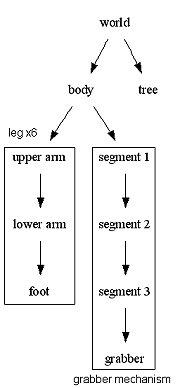
\includegraphics{forestwalkertree.png}
\end{center}
The tree structure for the forest walker shows the conceptual arrangement of observers and rigid bodies. This tree naturally follows from the connections between the moving bodies.%}}}

\section{Configuration Coordinates} %{{{

% Body {{{
The configuration of the observer $A_{Body}$ relative to the main observer $W$ can be described by a pure translation and a pure rotation where $c_i = \cos q_i$ and $s_i = \sin q_i$. The main forest walker body should be able to move freely with respect to the world, so it has six geometric degrees of freedom.

\begin{equation*}
r^{WA_{Body}} = w\left(\begin{array}{c}q_1\\q_2\\q_3\end{array}\right)
\end{equation*}

\begin{eqnarray*}
R_{wa^{(body)}} & = & R(q_4,1,0,0)R(q_5,0,1,0)R(q_6,0,0,1)\\
& = & \left(\begin{array}{ccc}
c_5c_6 & -c_5s_6 & s_5 \\
s_4s_5c_6+c_4s_6 & -s_4s_5s_6+c_4c_6 & -s_4c_5 \\
-c_4s_5c_6+s_4s_6 & c_4s_5s_6+s_4c_6 & c_4c_5
\end{array}\right)
\end{eqnarray*}
%}}}

% Leg {{{
Each leg $i$ can be described in relation to the body by comparing reference points and reference triads. Instead of describing each leg separately, we will generalize the translations and rotations and use $i$ from 1 through 6 to fully describe all of the legs.

% Upper Arm {{{
The upper arm is connected to the body such that

\begin{equation*}
r^{A_{Body}A_{UpperArm}} = a^{(body)}\left(\begin{array}{c}
p_{i1} \\ p_{i2} \\ p_{i3} \end{array}\right)\text{ and}
\end{equation*}

\begin{equation*}
R_{a^{(body)}a^{(upperarm)}} = R(q_{i1},0,1,0)R(q_{i2},1,0,0)\text{.}
\end{equation*}%}}}

% Lower Arm {{{
The configuration of the observer $A_{LowerArm}$ relative to the observer $A_{UpperArm}$ is described by

\begin{equation*}
r^{A_{UpperArm}A_{LowerArm}} = a^{(body)}\left(\begin{array}{c}
0 \\ 0 \\ \text{UpperArmLength} \end{array}\right)\text{ and}
\end{equation*}

\begin{equation*}
R_{a^{(upperarm)}a^{(lowerarm)}} = R(q_{i3},1,0,0)\text{.}
\end{equation*}%}}}

% Foot {{{
The configuration of the observer $A_{Foot}$ relative to the observer $A_{LowerArm}$ is described by a pure translation $T_{A_{LowerArm} \rightarrow A_{Foot}}$ corresponding to the position vector

\begin{equation*}
r^{A_{LowerArm}A_{Foot}}=a^{(lowerarm)}\left(\begin{array}{c}
0 \\ 0 \\ \text{LowerArmLength} \end{array}\right)
\end{equation*}

and a pure rotation $R_{A_{LowerArm} \rightarrow A_(Foot)}$ corresponding to the rotation matrix

\begin{equation*}
R_{a^{(lowerarm)}a^{(foot)}}=R(q_{i4},1,0,0)R(q_{i5},0,1,0) \text{.}
\end{equation*}%}}}
%}}}

% Grabber Mechanism {{{
The following will describe the tree grabber mechanism.

% Arm Segment 1 {{{
The configuration of the observer $A_{Arm1}$ relative to the observer $A_{Body}$ is described by a pure translation $T_{A_{Body} \rightarrow A_{Arm1}}$ corresponding to the position vector

\begin{equation*}
r^{A_{Body}A_{Arm1}}=a^{(body)}\left(\begin{array}{c}
0 \\ 0 \\ \text{BodyHeight}/2 \end{array}\right)
\end{equation*}

and a pure rotation $R_{a^{(body)} \rightarrow a^{(arm1)}}$ corresponding to the rotation matrix

\begin{equation*}
R_{a^{(body)}a^{(arm1)}}=R(q_7,0,0,1)R(q_8,0,0,1)\text{.}
\end{equation*}%}}}

% Arm Segment 2 {{{
The configuration of the observer $A_{Arm2}$ relative to the observer $A_{Arm1}$ is described by a pure translation $T_{A_{Arm1} \rightarrow A_{Arm2}}$ corresponding to the position vector

\begin{equation*}
r^{A_{Arm1}A_{Arm2}}=a^{(arm1)}\left(\begin{array}{c}
0 \\ 0 \\ \text{Arm1Length} \end{array}\right)
\end{equation*}

and a pure rotation $R_{a^{(arm1)} \rightarrow a^{(arm2)}}$ corresponding to the rotation matrix

\begin{equation*}
R_{a^{(arm1)}a^{(arm2)}}=R(q_9,1,0,0)\text{.}
\end{equation*}%}}}

% Arm Segment 3 {{{
The configuration of the observer $A_{Arm3}$ relative to the observer $A_{Arm2}$ is described by a pure translation $T_{A_{Arm2} \rightarrow A_{Arm3}}$ corresponding to the position vector

\begin{equation*}
r^{A_{Arm2}A_{Arm3}}=a^{(arm2)}\left(\begin{array}{c}
0 \\ 0 \\ \text{Arm2Length} \end{array}\right)
\end{equation*}

and a pure rotation $R_{a^{(arm2)} \rightarrow a^{(arm3)}}$ corresponding to the rotation matrix

\begin{equation*}
R_{a^{(arm2)}a^{(arm3)}}=R(q_{10},1,0,0)\text{.}
\end{equation*}%}}}

% Grabber {{{
The configuration of the observer $A_{Grabber}$ relative to the observer $A_{Arm3}$ is described by a pure translation $T_{A_{Arm3} \rightarrow A_{Grabber}}$ corresponding to the position vector

\begin{equation*}
r^{A_{Arm3}A_{Grabber}}=a^{(arm3)}\left(\begin{array}{c}
0 \\ 0 \\ \text{Arm3Length} + \text{GrabberDepth}/2 \end{array}\right)
\end{equation*}

and a pure rotation $R_{a^{(arm3)} \rightarrow a^{(grabber)}}$ corresponding to the rotation matrix

\begin{equation*}
R_{a^{(arm3)}a^{(grabber)}}=R(q_{11},1,0,0)\text{.}
\end{equation*}%}}}
%}}}

% Tree {{{
The configuration of the observer $A_{Tree}$ relative to the observer $W$ is described by a pure translation $T_{W \rightarrow A_{Tree}}$ corresponding to the position vector

\begin{equation*}
r^{WA_{Tree}}=w\left(\begin{array}{c}
q_{t1} \\ q_{t2} \\ q_{t3} \end{array}\right)
\end{equation*}

and a pure rotation $R_{w \rightarrow a^{(tree)}}$ corresponding to the rotation matrix

\begin{equation*}
R_{wa^{(tree)}}=R(q_{t4},0,0,1)R(q_{t5},1,0,0)R(q_{t6},0,0,1)\text{.}
\end{equation*}%}}}
%}}}

\section{Motion Constraints} %{{{
There are five constraints used in this animation. The first constrains the feet of the walker to always be flat with respect to the slope. The second constrains some of the walker's feet to the ground while its other feet are moving forward. The other three constraints are used in the dynamic portion of the animation. One is the gravitational force, attracting the tree downwards. Another is a repulsing force which keeps the tree from going through the slope, and the last is a frictional force on the log when it hits the hill.

% Feet constraints {{{
To keep the feet flat with respect to the ground, the $a_3^{(foot)}$ vector for each foot needs to be perpendicular to the slope. This constraint can be expressed by using the following two formulae for each foot $i$.

\begin{eqnarray*}
a_3^{(footi)} \cdot a_1^{(hill)} & = & 0 \\
a_3^{(footi)} \cdot a_3^{(hill)} & = & 0
\end{eqnarray*}

During some portions of the animation, some of the walker's feet need to be constrained to be at rest with respect to the ground. This is accomplished by making sure the linear velocity of the foot is 0.

\begin{eqnarray*}
{}^{Hill}v^{Footi} \cdot a_1^{(hill)} & = & 0 \\
{}^{Hill}v^{Footi} \cdot a_2^{(hill)} & = & 0 \\
{}^{Hill}v^{Footi} \cdot a_3^{(hill)} & = & 0 \\
\end{eqnarray*}

However, it must be kept in mind that these five equations apply to all six of the walker's legs, resulting in a total of 30 constraints.%}}}

% Tree constraints {{{
The dynamics portion of the animation requires three different types of constraints. However, they can all be considered a single constraint on the force being applied to the falling log. The force of gravity can be represented by the vector

\begin{equation*}
F_g = w\left(\begin{array}{c} 0 \\ 0 \\ -Mg \end{array}\right)\text{.}
\end{equation*}

This force is always applied to the tree. The second force is the repulsive force applied by the hill to the tree. This is always normal to the hill with a magnitude dependent on the tree's penetration into the slope.

\begin{equation*}
F_r = \text{scale}\left(a_3^{(hill)}\right)
\end{equation*}

This force is only applied at the ends of the log, and only when the log is bouncing against the hill. The last force is the frictional force applied when the log is hitting the hill. This is proportional to the normal force applied from the hill to the log, which happens to also be the repulsive force being applied to the log. 

\begin{equation*}
F_f = 0.1F_r
\end{equation*}

Therefore, the tree's constraints will be applied through the equation $F = F_g + F_r + F_f$ for force and $T = F-r$ for an applied torque. These will need to be split up to become valid differential equations:

\begin{eqnarray*}
\left(F - F_g - F_r - F_f\right) \cdot w_1 & = & 0 \\
\left(F - F_g - F_r - F_f\right) \cdot w_2 & = & 0 \\
\left(F - F_g - F_r - F_f\right) \cdot w_3 & = & 0 \\
\left(T - F_r\right) \cdot w_1 & = & 0 \\
\left(T - F_r\right) \cdot w_2 & = & 0 \\
\left(T - F_r\right) \cdot w_3 & = & 0
\end{eqnarray*}%}}}
%}}}

\section{Kinematic Differential Equations} %{{{
We turn to the selection of independent velocity coordinates to uniquely specify all allowable motions of the walker. There are six dynamic degrees of freedom for the walker, and three dynamic degrees of freedom for each leg. Combined with five degrees for the grabber mechanism, there are 29 total dynamic degrees of freedom.

We control the walker by moving the body, selectively constraining particular feet to the ground while moving the other feet to create the illusion of a walking motion. Because only three feet move at a time, the independent velocity coordinates are whittled down to 20. However, we can reduce this even further by realizing that the three feet which move at a time move at the same velocity; this allows us to use only three coordinates to move the feet and gives us 14 independent coordinates.

We arrive at the following set of kinematic differential equations for moving the body:

\begin{eqnarray*}
{}^{Hill}v^{Body} \cdot a_1^{(hill)} & = & u_1 \\
{}^{Hill}v^{Body} \cdot a_2^{(hill)} & = & u_2 \\
{}^{Hill}v^{Body} \cdot a_3^{(hill)} & = & u_3 \\
{}^{a^{(hill}}\omega^{a^{(body)}} \cdot a_1^{(hill)} & = & u_4 \\
{}^{a^{(hill}}\omega^{a^{(body)}} \cdot a_2^{(hill)} & = & u_5 \\
{}^{a^{(hill}}\omega^{a^{(body)}} \cdot a_3^{(hill)} & = & u_6
\end{eqnarray*}

The legs are alternatively constrained or utilized through the following kinematic differential equations, repeated once for each leg. The choice of using either coordinate depends on which leg the set of equations represents.

\begin{eqnarray*}
a_3^{(footi)} \cdot a_1^{(hill)} & = & 0 \\
a_3^{(footi)} \cdot a_3^{(hill)} & = & 0 \\
{}^{Hill}v^{Footi} \cdot a_1^{(hill)} & = & (case)u_7 \text{ or } (case)u_{10} \\
{}^{Hill}v^{Footi} \cdot a_2^{(hill)} & = & (case)u_8 \text{ or } (case)u_{11} \\
{}^{Hill}v^{Footi} \cdot a_3^{(hill)} & = & (case)u_9 \text{ or } (case)u_{12}
\end{eqnarray*}

Lastly, there are five equations for the grabber mechanism.

\begin{eqnarray*}
{}^{a^{(body)}}\omega^{a^{(arm1)}} \cdot a_3^{(arm1)} & = & u_{13} \\
{}^{a^{(body)}}\omega^{a^{(arm1)}} \cdot a_1^{(arm1)} & = & u_{14} \\
{}^{a^{(arm1)}}\omega^{a^{(arm2)}} \cdot a_1^{(arm1)} & = & u_{15} \\
{}^{a^{(arm2)}}\omega^{a^{(arm3)}} \cdot a_1^{(arm1)} & = & u_{16} \\
{}^{a^{(arm3)}}\omega^{a^{(grabber)}} \cdot a_1^{(arm1)} & = & u_{16}
\end{eqnarray*}

Singularities exist in this set of equations. When the legs are constrained to the slope, the body cannot be moved farther than the legs can reach without causing a singularity.

However, the tree also requires a set of kinematic differential equations. As it is unconstrained, the equations which apply to the tree are very similar:

\begin{eqnarray*}
{}^{Hill}v^{Tree} \cdot a_1^{(w)} & = & u_1 \\
{}^{Hill}v^{Tree} \cdot a_2^{(w)} & = & u_2 \\
{}^{Hill}v^{Tree} \cdot a_3^{(w)} & = & u_3 \\
{}^{a^{(w}}\omega^{a^{(tree)}} \cdot a_1^{(tree)} & = & u_4 \\
{}^{a^{(w}}\omega^{a^{(tree)}} \cdot a_2^{(tree)} & = & u_5 \\
{}^{a^{(w}}\omega^{a^{(tree)}} \cdot a_3^{(tree)} & = & u_6
\end{eqnarray*}%}}}

\section{Dynamic Differential Equations} %{{{
The forces acting on the dropped tree can now be defined through dynamic differential equations. There are no outside forces acting on the tree, so it is dynamically completely constrained. Thus, the dynamic differential equations follow.

\begin{eqnarray*}
\left(F - F_g - F_r - F_f\right) \cdot w_1 & = & 0 \\
\left(F - F_g - F_r - F_f\right) \cdot w_2 & = & 0 \\
\left(F - F_g - F_r - F_f\right) \cdot w_3 & = & 0 \\
\left(T - F_r\right) \cdot w_1 & = & 0 \\
\left(T - F_r\right) \cdot w_2 & = & 0 \\
\left(T - F_r\right) \cdot w_3 & = & 0
\end{eqnarray*}
%}}}

\section{MAMBO} %{{{

\begin{verbatim}
maple(['DeclareObservers(W,ABody,Tree,Hill,'...
	'seq(cat(ALeg,i,UpperArm),i=1..6),'...
	'seq(cat(ALeg,i,LowerArm),i=1..6),'...
	'seq(cat(AFoot,i),i=1..6))']);
maple(['DeclarePoints(W,ABody,Tree,Hill,Tree1,Tree2,'...
	'seq(cat(ALeg,i,UpperArm),i=1..6),'...
	'seq(cat(ALeg,i,LowerArm),i=1..6),'...
	'seq(cat(AFoot,i),i=1..6),'...
	'seq(cat(ALeg,i,UpperArmEnd),i=1..6),'...
	'seq(cat(ALeg,i,LowerArmEnd),i=1..6))']);
maple(['DeclareTriads(w,aBody,tree,hill,'...
	'seq(cat(aLeg,i,UpperArm),i=1..6),'...
	'seq(cat(aLeg,i,LowerArm),i=1..6),'...
	'seq(cat(aFoot,i),i=1..6))']);

maple(['DefineNeighbors([W,Tree],[W,Hill],[Hill,ABody],'...
	'seq([ABody,cat(ALeg,i,UpperArm)],i=1..6),'...
	'seq([cat(ALeg,i,UpperArm),cat(ALeg,i,LowerArm)],i=1..6),'...
	'seq([cat(ALeg,i,LowerArm),cat(AFoot,i)],i=1..6))']);

maple(['DefineTriads('...
    '[w,tree,[qd4,3],[qd5,1],[qd6,3]],'...
    '[w,hill,[pd4,3],[pd5,1],[pd6,3]])']);

maple(['DefineTriads([hill,aBody,[q4,1],[q5,2],[q6,3]],'...
	'seq([aBody,cat(aLeg,i,UpperArm),[cat(q,i,1),2],[cat(q,i,2),1]],i=1..6),'...
	'seq([cat(aLeg,i,UpperArm),cat(aLeg,i,LowerArm),cat(q,i,3),1],i=1..6),'...
	'seq([cat(aLeg,i,LowerArm),cat(aFoot,i),[cat(q,i,4),1],[cat(q,i,5),2]],i=1..6))']);

maple(['DefineObservers('...
	'[W,W,w],[ABody,ABody,aBody],[Tree,Tree,tree],[Hill,Hill,hill],'...
	'seq([cat(ALeg,i,UpperArm),cat(ALeg,i,UpperArm),cat(aLeg,i,UpperArm)],i=1..6),'...
	'seq([cat(ALeg,i,LowerArm),cat(ALeg,i,LowerArm),cat(aLeg,i,LowerArm)],i=1..6),'...
	'seq([cat(AFoot,i),cat(AFoot,i),cat(aFoot,i)],i=1..6))']);

maple('Scalar:=2.0');
maple('Scalar2:=0.4');
maple('LengthUpperArm:=Scalar2 * 7');
maple('LengthKnee:=Scalar2 * 2');
maple('LengthLowerArm:=Scalar2 * 8');

maple(['DefinePoints([W,Tree,w,qd1,qd2,qd3],'...
    '[Tree,Tree1,tree,0,0,L/2],'...
    '[Tree,Tree2,tree,0,0,-L/2],'...
    '[W,Hill,w,pd1,pd2,pd3])']);

maple(['bodyBaseLength:=10;'...
	'bodyBaseHeight:=0.25;'...
	'bodyBaseWidth:=1.5;'...
	'engineBaseLength:=bodyLength/2;'...
	'engineBaseHeight:=bodyHeight;'...
	'engineBaseWidth:=bodyWidth;'...
	'axisLength:=bodyWidth + 1.90;'...
	'axisWidth:=1;'...
	'axisHeight:=axisWidth;'...
	'engineBlockMiddleHeight:=2;'...
	'engineBlockMiddleLength:=2.5;'...
	'engineBlockMiddleWidth:=bodyBaseWidth+0.5;'...
	'thoraxLength:=2.399;'...
	'thoraxHeight:=2;'...
	'thoraxWidth:=bodyBaseWidth+0.5']);
    
maple(['DefinePoints('...
	'[Hill,ABody,hill,q1,q2,q3],'...
	'[ABody,ALeg1UpperArm,aBody,axisLength/2 + 0.4,axisHeight/2+0.5,1.35],'...
	'[ABody,ALeg2UpperArm,aBody,axisLength/2 + 0.4,axisHeight+0.5,-0.35],'...
	'[ABody,ALeg3UpperArm,aBody,axisLength/2 + 0.4,axisHeight/2+0.5,-4.5],'...
	'[ABody,ALeg4UpperArm,aBody,-axisLength/2 - 0.4,axisHeight/2+0.5,1.35],'...
	'[ABody,ALeg5UpperArm,aBody,-axisLength/2 - 0.4,axisHeight+0.5,-0.35],'...
	'[ABody,ALeg6UpperArm,aBody,-axisLength/2 - 0.4,axisHeight/2+0.5,-4.5],'...
	'seq([cat(ALeg,i,UpperArm),cat(ALeg,i,UpperArmEnd),cat(aLeg,i,UpperArm),0,0,LengthUpperArm],i=1..6),'...
	'seq([cat(ALeg,i,UpperArmEnd),cat(ALeg,i,LowerArm),cat(aLeg,i,UpperArm),0,0,0],i=1..6),'...
	'seq([cat(ALeg,i,LowerArm),cat(ALeg,i,LowerArmEnd),cat(aLeg,i,LowerArm),0,0,LengthLowerArm],i=1..6),'...
	'seq([cat(ALeg,i,LowerArmEnd),cat(AFoot,i),cat(aLeg,i,LowerArm),0,0,0],i=1..6))']);

% Make the tree drop
maple('DeclareStates(qd1,qd2,qd3,qd4,qd5,qd6,ud1,ud2,ud3,ud4,ud5,ud6)');
maple(['kdeT:={seq(LinearVelocity(W,Tree) &oo MakeTranslations(w,i)=cat(ud,i),i=1..3),'...
    'seq(AngularVelocity(w,tree) &oo MakeTranslations(tree,i)=cat(ud,i+3),i=1..3)}']);

maple('p:=subs(kdeT,LinearMomentum(W,Tree))');
maple('h:=subs(kdeT,AngularMomentum(W,tree))');

maple('depth1:=FindTranslation(Hill,Tree1) &oo MakeTranslations(hill,3)');
maple('depth2:=FindTranslation(Hill,Tree2) &oo MakeTranslations(hill,3)');

maple('gravity:=(caset &** MakeTranslations(w,0,0,-M*g))');
maple('normal1:= (-scale * depth1) &** MakeTranslations(hill,3)');
maple('normal2:= (-scale * depth2) &** MakeTranslations(hill,3)');
maple('vel:=subs(kdeT,LinearVelocity(Hill,Tree))');
maple('friction:= (0.1/VectorLength(vel)) &** vel');

maple('force1:= normal1 &++ (VectorLength(normal1) &** friction)');
maple('force2:= normal2 &++ (VectorLength(normal2) &** friction)');

maple('r1:=FindTranslation(Tree,Tree1)');
maple('r2:=FindTranslation(Tree,Tree2)');

maple('a:=0.343');
maple('c:=0.020');

maple(['ddeT:={'...
    'seq((DiffTime(p,w) &-- gravity'...
        '&-- ((1 - case1) &** force1)'...
        '&-- ((1 - case2) &** force2))'...
        '&oo MakeTranslations(w,i)=0,i=1..3),'...
    'seq((DiffTime(h,w)'...
        '&-- ((1 - case1) &** (r1 &xx force1))'...
        '&-- ((1 - case2) &** (r2 &xx force2)))'...
        '&oo MakeTranslations(w,i)=0,i=1..3)}']);

%----------------------------------------------------------------------------
%----------------------------------------------------------------------------
%----------------------------------------------------------------------------
% LEGS

% Thigh
maple(['DefineObjects('...
	'seq([cat(ALeg,i,UpperArm),''Cylinder'',point=cat(ALeg,i,UpperArm),orient=MakeRotations(90 * 3.14159/180,0,1,0),radius=0.5,length=0.8],i=1..6))'...
	'seq([cat(ALeg,i,UpperArm),''Block'',point=MakeTranslations(cat(aLeg,i,UpperArm),0,0,LengthUpperArm/2),zlength=LengthUpperArm,ylength=1,xlength=0.8],i=1..6))'...
	'seq([cat(ALeg,i,UpperArm),''Cylinder'',point=cat(ALeg,i,UpperArmEnd),orient=MakeRotations(90 * 3.14159/180,0,1,0),radius=0.5,length=0.8],i=1..6))']);

% Lower Leg
maple(['DefineObjects('...
	'seq([cat(ALeg,i,LowerArm),''Block'',point=MakeTranslations(cat(aLeg,i,LowerArm),0,0,LengthLowerArm/2),zlength=LengthLowerArm,ylength=0.5,xlength=0.6],i=1..6))']);

% Foot
maple(['DefineObjects('...
	'seq([cat(AFoot,i),''Cylinder'',orient=w,length=0.1,radius=0.5,color="{1,0,0}"],i=1..6))']);

% Draw the Tree
maple(['DefineObjects([Tree,''Cylinder'',length=L,radius=R,color="{0.55,0.27,0.07}"],'...
    '[Hill,''Block'',xlength=1000,ylength=1000,zlength=.01,color="{0,0.39,0}"])']);

maple('DeclareStates(seq(cat(q,k),k=1..6),seq(seq(cat(q,i,j),j=1..5),i=1..6))');

%Walker Grabber Arm Declares
maple('DeclarePoints(A1,A2,A3,A4)');
maple('DeclareObservers(A1,A2,A3,A4)');
maple('DeclareTriads(a1,a2,a3,a4)');

%Walker Grabber Declares
maple('DeclarePoints(G1)');
maple('DeclareObservers(G1)');

%Walker Grabber Arm Defines
maple('DefineObservers([A1,A1,a1],[A2,A2,a2],[A3,A3,a3],[A4,A4,a4])');
maple('DefineNeighbors([ABody,A1],[A1,A2],[A2,A3],[A3,A4])');
maple('DefineTriads(aBody,a1,[q_7,1],[q_8,3])');
maple('DefineTriads(a1,a2,q_9,1)');
maple('DefineTriads(a2,a3,q_10,1)');
maple('DefineTriads(a3,a4,q_11,1)');
maple('DefinePoints([ABody,A1,aBody,0,heightBody/2,0],[A1,A2,a1,0,0,p1],[A2,A3,a2,0,0,p2],[A3,A4,a3,0,0,p3])');

%Walker Grabber Defines
maple('DefineObservers([G1,G1,a4])');
maple('DefineNeighbors([A4,G1])');
maple('DefinePoints([A4,G1,a4,0,0,p4])');

maple('BodyInset:=Scalar * 0.002');


%------------------------------------------------------------------------

% base of the walker-body
maple(['DefineObjects('...
	'[ABody,''Block'',point=ABody,orient=aBody,zlength=bodyBaseLength,ylength=bodyBaseHeight,xlength=bodyBaseWidth,color="{0.2,0.2,0.2}"],'...
	'[ABody,''Block'',point=MakeTranslations(aBody,0,0,-bodyBaseLength/2),orient=aBody,zlength=engineBaseLength,ylength=engineBaseHeight,xlength=engineBaseWidth,color="{0.2,0.2,0.2}"],'...
	'[ABody,''Block'',point=MakeTranslations(aBody,bodyBaseWidth/2,0,bodyBaseLength/2 - 2.236067977/2),orient=MakeRotations(-26.56505118 * PI/180,0,1,0),zlength=2,ylength=bodyBaseHeight,xlength=1,color="{0.2,0.2,0.2}"],'...
	'[ABody,''Block'',point=MakeTranslations(aBody,-bodyBaseWidth/2,0,bodyBaseLength/2 - 2.236067977/2),orient=MakeRotations(26.56505118 * PI/180,0,1,0),zlength=2,ylength=bodyBaseHeight,xlength=1,color="{0.2,0.2,0.2}"],'...
	'[ABody,''Block'',point=MakeTranslations(aBody,bodyBaseWidth/2+0.4472135955,0,-(bodyBaseLength/4+1.788854382)/2),orient=aBody,zlength=(bodyBaseLength+engineBaseLength/2-1.788854382),ylength=bodyBaseHeight,xlength=0.894427191,color="{0.2,0.2,0.2}"],'...
	'[ABody,''Block'',point=MakeTranslations(aBody,-(bodyBaseWidth/2+0.4472135955),0,-(bodyBaseLength/4+1.788854382)/2),orient=aBody,zlength=(bodyBaseLength+engineBaseLength/2-1.788854382),ylength=bodyBaseHeight,xlength=0.894427191,color="{0.2,0.2,0.2}"])']);

% connection axes for legs
maple(['DefineObjects('...
	'[ABody,''Block'',point=MakeTranslations(aBody,0,axisHeight/2+0.5,1.35),orient=MakeRotations(PI/2,0,1,0),zlength=axisLength,ylength=axisHeight,xlength=axisWidth,color="{0.2,0.2,0.2}"],'...
	'[ABody,''Block'',point=MakeTranslations(aBody,0,axisHeight+0.5,-0.35),orient=MakeRotations(PI/2,0,1,0),zlength=axisLength,ylength=axisHeight,xlength=axisWidth,color="{0.2,0.2,0.2}"],'...
	'[ABody,''Block'',point=MakeTranslations(aBody,0,axisHeight/2+0.5,-4.5),orient=MakeRotations(PI/2,0,1,0),zlength=axisLength,ylength=axisHeight,xlength=axisWidth,color="{0.2,0.2,0.2}"])']);

% engine block
maple(['DefineObjects('...
	'[ABody,''Block'',point=MakeTranslations(aBody,0,engineBlockMiddleHeight/2,-bodyBaseLength/2),orient=aBody,zlength=engineBlockMiddleLength,ylength=engineBlockMiddleHeight,xlength=engineBlockMiddleWidth,color="{0.2,0.2,0.2}"],'...
	'[ABody,''Block'',point=MakeTranslations(aBody,0,1,-6.75),orient=MakeRotations(-30 * PI/180,1,0,0),zlength=1.7,ylength=1.2,xlength=bodyBaseWidth,color="{0.2,0.2,0.2}"],'...
	'[ABody,''Block'',point=MakeTranslations(aBody,0,0.5,-6.75),orient=aBody,zlength=1,ylength=1,xlength=bodyBaseWidth,color="{0.2,0.2,0.2}"],'...
	'[ABody,''Block'',point=MakeTranslations(aBody,0,1.1,-3.5),orient=aBody,zlength=0.5,ylength=2.2,xlength=bodyBaseWidth+1,color="{0.2,0.2,0.2}"],'...
	'[ABody,''Block'',point=MakeTranslations(aBody,0,0.55,-2.70),orient=aBody,zlength=1.1,ylength=1.1,xlength=bodyBaseWidth+1,color="{0.2,0.2,0.2}"],'...
	'[ABody,''Block'',point=MakeTranslations(aBody,0,0.7,-2.94),orient=aBody,zlength=1.1,ylength=1.1,xlength=bodyBaseWidth+1,color="{0.2,0.2,0.2}"],'...
	'[ABody,''Block'',point=MakeTranslations(aBody,0,1.42,-2.94),orient=MakeRotations(PI/4,1,0,0),zlength=1.555,ylength=0.7,xlength=bodyBaseWidth+1,color="{0.2,0.2,0.2}"])']);

% thorax region
maple(['DefineObjects('...
	'[ABody,''Block'',point=MakeTranslations(aBody,0,thoraxHeight/2,-(thoraxLength - 0.5)/2),orient=aBody,zlength=thoraxLength,ylength=thoraxHeight,xlength=thoraxWidth,color="{0.2,0.2,0.2}"])']);
	
% cab
maple(['DefineObjects('...
	'[ABody,''Block'',point=MakeTranslations(aBody,bodyBaseWidth/2 + 0.333,0.377,bodyBaseLength/2 - 2.236067977/2 + 0.165),orient=MakeRotations(-26.56505118 * PI/180,0,1,0),zlength=2,ylength=1,xlength=0.25,color="{0,0.5,0}"],'...
	'[ABody,''Block'',point=MakeTranslations(aBody,-bodyBaseWidth/2 - 0.333,0.377,bodyBaseLength/2 - 2.236067977/2 + 0.165),orient=MakeRotations(26.56505118 * PI/180,0,1,0),zlength=2,ylength=1,xlength=0.25,color="{0,0.5,0}"],'...
	'[ABody,''Block'',point=MakeTranslations(aBody,0,0.377,bodyBaseLength/2 - 0.126),orient=aBody,zlength=0.25,ylength=1,xlength=bodyBaseWidth,color="{0,0.5,0}"],'...
	'[ABody,''Block'',point=MakeTranslations(aBody,1.227,0.377,2.900),orient=MakeRotations(40 * PI/180,0,1,0),zlength=1,ylength=1,xlength=0.25,color="{0,0.5,0}"],'...
	'[ABody,''Block'',point=MakeTranslations(aBody,-1.227,0.377,2.900),orient=MakeRotations(-40 * PI/180,0,1,0),zlength=1,ylength=1,xlength=0.25,color="{0,0.5,0}"],'...
	'[ABody,''Block'',point=MakeTranslations(aBody,0,0.877,1.50),orient=aBody,zlength=2.5,ylength=2.0,xlength=2.0,color="{0,0.5,0}"],'...
	'[ABody,''Block'',point=MakeTranslations(aBody,1.1,1,2.75),orient=MakeRotations([40 * PI/180,0,1,0],[60 * PI/180,1,0,0]),zlength=1,ylength=1,xlength=0.25,color="{0,0.5,0}"],'...
	'[ABody,''Block'',point=MakeTranslations(aBody,-1.1,1,2.75),orient=MakeRotations([-40 * PI/180,0,1,0],[60 * PI/180,1,0,0]),zlength=1,ylength=1,xlength=0.25,color="{0,0.5,0}"],'...
	'[ABody,''Block'',point=MakeTranslations(aBody,0,1.650,4.375),orient=MakeRotations(-30 * PI/180,1,0,0),zlength=0.25,ylength=2.0,xlength=bodyBaseWidth,color="{0.5,0.5,1}"],'...
	'[ABody,''Block'',point=MakeTranslations(aBody,0,2.97,3.055),orient=MakeRotations(-60 * PI/180,1,0,0),zlength=0.25,ylength=2.0,xlength=bodyBaseWidth,color="{0.5,0.5,1}"],'...
	'[ABody,''Block'',point=MakeTranslations(aBody,0,3.45,1.875),orient=MakeRotations(90 * PI/180,1,0,0),zlength=0.25,ylength=0.75,xlength=bodyBaseWidth,color="{0.5,0.5,1}"],'...
	'[ABody,''Block'',point=MakeTranslations(aBody,0,2.65,1.1),orient=MakeRotations(30 * PI/180,1,0,0),zlength=0.25,ylength=2,xlength=bodyBaseWidth,color="{0.5,0.5,1}"])']);

%Walker Grabber Arm Objects
maple('DefineObjects(seq([cat(A,i),''Sphere'',point=cat(A,i),radius=0.25,color="{71/255,71/255,71/255}"],i=1..4))');
maple('DefineObjects(seq([cat(A,i),''Cylinder'',point=0.5 &** FindTranslation(cat(A,i),cat(A,i+1)), radius=0.25, length=cat(p,i),color="{71/255,71/255,71/255}"],i=1..3))');

%Walker Grabber Objects
maple('DefineObjects([G1,''Block'',xlength=p4*1.5,ylength=p4/2.5,zlength=p4*2,color=yellow])');
maple('DefineObjects([G1,''Cylinder'',orient = MakeRotations([1.571,1]),point=MakeTranslations([a4,p4/1.5,p4/3,0]),radius=p4/2,length=p4/2.5,color="{71/255,71/255,71/255}"])');
maple('DefineObjects([G1,''Cylinder'',orient = MakeRotations([1.571,1]),point=MakeTranslations([a4,-p4/1.5,p4/3,0]),radius=p4/2,length=p4/2.5,color="{71/255,71/255,71/255}"])');


maple('DeclareStates(seq(cat(q_,i),i=7..11))');

% Constrain the feet
maple('f1:=MakeTranslations(aFoot1,3) &oo MakeTranslations(hill,1)=0');
maple('f2:=MakeTranslations(aFoot1,3) &oo MakeTranslations(hill,3)=0');
maple('f13:=LinearVelocity(Hill,AFoot1) &oo MakeTranslations(hill,1)=(1-case)*u10');
maple('f14:=LinearVelocity(Hill,AFoot1) &oo MakeTranslations(hill,2)=(1-case)*u11');
maple('f15:=LinearVelocity(Hill,AFoot1) &oo MakeTranslations(hill,3)=(1-case)*u12');

maple('f3:=MakeTranslations(aFoot2,3) &oo MakeTranslations(hill,1)=0');
maple('f4:=MakeTranslations(aFoot2,3) &oo MakeTranslations(hill,3)=0');
maple('f16:=LinearVelocity(Hill,AFoot2) &oo MakeTranslations(hill,1)=case*u7');
maple('f17:=LinearVelocity(Hill,AFoot2) &oo MakeTranslations(hill,2)=case*u8');
maple('f18:=LinearVelocity(Hill,AFoot2) &oo MakeTranslations(hill,3)=case*u9');

maple('f5:=MakeTranslations(aFoot3,3) &oo MakeTranslations(hill,1)=0');
maple('f6:=MakeTranslations(aFoot3,3) &oo MakeTranslations(hill,3)=0');
maple('f19:=LinearVelocity(Hill,AFoot3) &oo MakeTranslations(hill,1)=(1-case)*u7');
maple('f20:=LinearVelocity(Hill,AFoot3) &oo MakeTranslations(hill,2)=(1-case)*u8');
maple('f21:=LinearVelocity(Hill,AFoot3) &oo MakeTranslations(hill,3)=(1-case)*u9');

maple('f7:=MakeTranslations(aFoot4,3) &oo MakeTranslations(hill,1)=0');
maple('f8:=MakeTranslations(aFoot4,3) &oo MakeTranslations(hill,3)=0');
maple('f22:=LinearVelocity(Hill,AFoot4) &oo MakeTranslations(hill,1)=case*u10');
maple('f23:=LinearVelocity(Hill,AFoot4) &oo MakeTranslations(hill,2)=case*u11');
maple('f24:=LinearVelocity(Hill,AFoot4) &oo MakeTranslations(hill,3)=case*u12');

maple('f9:=MakeTranslations(aFoot5,3) &oo MakeTranslations(hill,1)=0');
maple('f10:=MakeTranslations(aFoot5,3) &oo MakeTranslations(hill,3)=0');
maple('f25:=LinearVelocity(Hill,AFoot5) &oo MakeTranslations(hill,1)=(1-case)*u7');
maple('f26:=LinearVelocity(Hill,AFoot5) &oo MakeTranslations(hill,2)=(1-case)*u8');
maple('f27:=LinearVelocity(Hill,AFoot5) &oo MakeTranslations(hill,3)=(1-case)*u9');

maple('f11:=MakeTranslations(aFoot6,3) &oo MakeTranslations(hill,1)=0');
maple('f12:=MakeTranslations(aFoot6,3) &oo MakeTranslations(hill,3)=0');
maple('f28:=LinearVelocity(Hill,AFoot6) &oo MakeTranslations(hill,1)=case*u7');
maple('f29:=LinearVelocity(Hill,AFoot6) &oo MakeTranslations(hill,2)=case*u8');
maple('f30:=LinearVelocity(Hill,AFoot6) &oo MakeTranslations(hill,3)=case*u9');

maple(['kde:={'...
        'LinearVelocity(Hill,ABody) &oo MakeTranslations(hill,1)=u1,'...
        'LinearVelocity(Hill,ABody) &oo MakeTranslations(hill,2)=u2,'...
        'LinearVelocity(Hill,ABody) &oo MakeTranslations(hill,3)=u3,'...
        'AngularVelocity(hill,aBody) &oo MakeTranslations(hill,1)=u4,'...
        'AngularVelocity(hill,aBody) &oo MakeTranslations(hill,2)=u5,'...
        'AngularVelocity(hill,aBody) &oo MakeTranslations(hill,3)=u6}'...
        'union DiffTime({f1,f2,f3,f4,f5,f6,f7,f8,f9,f10,f11,f12})'...
        'union {seq(cat(f,i),i=13..30)} union {seq(cat(q_,i,t)=cat(u_,i),i=7..11)}']);

maple(['GeometryOutput(main=W,'...
'states=[qd1,qd2,qd3,qd4,qd5,qd6,'...
'ud1,ud2,ud3,ud4,ud5,ud6,case1,case2,'...
'q1,q2,q3,q4,q5,q6,'...
'q_7,q_8,q_9,q_10,q_11,'...
'q11,q12,q13,q14,q15,'...
'q21,q22,q23,q24,q25,'...
'q31,q32,q33,q34,q35,'...
'q41,q42,q43,q44,q45,'...
'q51,q52,q53,q54,q55,'...
'q61,q62,q63,q64,q65],'...
'parameters=[heightBody,lengthBody,widthBody,p1,p2,p3,p4,'...
'pd1,pd2,pd3,pd4,pd5,pd6,seq(seq(cat(Inertia,i,j),i=1..3),j=1..3),'...
'L,R,M,g,scale],checkargs,'...
'filename="ForestWalker.geo")']);

maple(['MotionOutput(ode=kde union kdeT union ddeT,'...
'states=['...
'qd1,qd2=-16.75,qd3=5,qd4,qd5=.01,qd6,'...
'ud1,ud2=-1,ud3,ud4,ud5,ud6,'...
'q1,q2,q3=1.8,q4=1.5708,q5,q6,'...
'q_7=-1.57079,q_8,q_9=1,q_10=1,q_11=1.1,'...
'q11,q12=-0.17,q13=1.75,q14,q15,'...
'q21,q22=-3.17,q23=-1.5,q24=-0.2,q25,'...
'q31,q32=-3,q33=-1.5,q34=-0.2,q35,'...
'q41,q42=-0.17,q43=1.75,q44,q45,'...
'q51,q52=-3.17,q53=-1.5,q54=-0.2,q55,'...
'q61,q62=-3,q63=-1.5,q64=-0.2,q65],'...
'parameters=['...
'heightBody=2.6,lengthBody=15.6,widthBody=5.2,'...
'p1=4,p2=10,p3=8,p4=1.5,'...
'pd1,pd2,pd3=-3.5,pd4,pd5=0.05,pd6,'...
'Inertia11=a,Inertia12,Inertia13,Inertia21,Inertia22=a,Inertia23,Inertia31,Inertia32,Inertia33=c,'...
'L=4,R=0.25,M=1,g=10,scale=10000,Pi=3.14159],'...
'insignals=['...
'case1=(depth1&>0),case2=(depth2&>0),'...
'case=(sin(Pi*t)&>0),'...
'caset=(t&>2),'...
'u_7=0,u_8=0,u_9=0,u_10=0,u_11=0,'...
'u1=0,u2=-1,u3=0,u4=0,u5=0,u6=0,'...
'u7=0,u8=-2,u9=2*(sin(Pi*2*t)),'...
'u10=0,u11=-2,u12=2*(sin(Pi*2*t))],'...
'checkargs,filename="ForestWalker.dyn")']);
\end{verbatim}

\end{document}

